\documentclass[11pt]{article}\usepackage[]{graphicx}\usepackage[]{color}
%% maxwidth is the original width if it is less than linewidth
%% otherwise use linewidth (to make sure the graphics do not exceed the margin)
\makeatletter
\def\maxwidth{ %
  \ifdim\Gin@nat@width>\linewidth
    \linewidth
  \else
    \Gin@nat@width
  \fi
}
\makeatother

\definecolor{fgcolor}{rgb}{0.345, 0.345, 0.345}
\newcommand{\hlnum}[1]{\textcolor[rgb]{0.686,0.059,0.569}{#1}}%
\newcommand{\hlstr}[1]{\textcolor[rgb]{0.192,0.494,0.8}{#1}}%
\newcommand{\hlcom}[1]{\textcolor[rgb]{0.678,0.584,0.686}{\textit{#1}}}%
\newcommand{\hlopt}[1]{\textcolor[rgb]{0,0,0}{#1}}%
\newcommand{\hlstd}[1]{\textcolor[rgb]{0.345,0.345,0.345}{#1}}%
\newcommand{\hlkwa}[1]{\textcolor[rgb]{0.161,0.373,0.58}{\textbf{#1}}}%
\newcommand{\hlkwb}[1]{\textcolor[rgb]{0.69,0.353,0.396}{#1}}%
\newcommand{\hlkwc}[1]{\textcolor[rgb]{0.333,0.667,0.333}{#1}}%
\newcommand{\hlkwd}[1]{\textcolor[rgb]{0.737,0.353,0.396}{\textbf{#1}}}%

\usepackage{framed}
\makeatletter
\newenvironment{kframe}{%
 \def\at@end@of@kframe{}%
 \ifinner\ifhmode%
  \def\at@end@of@kframe{\end{minipage}}%
  \begin{minipage}{\columnwidth}%
 \fi\fi%
 \def\FrameCommand##1{\hskip\@totalleftmargin \hskip-\fboxsep
 \colorbox{shadecolor}{##1}\hskip-\fboxsep
     % There is no \\@totalrightmargin, so:
     \hskip-\linewidth \hskip-\@totalleftmargin \hskip\columnwidth}%
 \MakeFramed {\advance\hsize-\width
   \@totalleftmargin\z@ \linewidth\hsize
   \@setminipage}}%
 {\par\unskip\endMakeFramed%
 \at@end@of@kframe}
\makeatother

\definecolor{shadecolor}{rgb}{.97, .97, .97}
\definecolor{messagecolor}{rgb}{0, 0, 0}
\definecolor{warningcolor}{rgb}{1, 0, 1}
\definecolor{errorcolor}{rgb}{1, 0, 0}
\newenvironment{knitrout}{}{} % an empty environment to be redefined in TeX

\usepackage{alltt}

\usepackage{amssymb,amsmath}
\usepackage{enumerate}
\usepackage{float}
\usepackage{verbatim}
\usepackage{setspace}
\usepackage{multicol}

%% LaTeX margin settings:
  \setlength{\textwidth}{7.0in}
\setlength{\textheight}{9in}
\setlength{\oddsidemargin}{-.5in}
\setlength{\evensidemargin}{0in}
\setlength{\topmargin}{-1.5cm}

%% tell knitr to use smaller font for code chunks
\def\fs{\footnotesize}
\def\R{{\sf R}}
\newcommand{\bfbeta}{\mbox{\boldmath $\beta$}}
\newcommand{\bfD}{\mbox{\boldmath $D$}}
\newcommand{\bfL}{\mbox{\boldmath $L$}}
\newcommand{\bfR}{\mbox{\boldmath $R$}}
\newcommand{\bfmu}{\mbox{\boldmath $\mu$}}
\newcommand{\bfv}{\mbox{\boldmath $V$}}
\newcommand{\bfX}{\mbox{\boldmath $X$}}
\newcommand{\bfy}{\mbox{\boldmath $y$}}
\newcommand{\bfb}{\mbox{\boldmath $b$}}
\newcommand{\ytil}{\mbox{$\tilde{y}$}}
\IfFileExists{upquote.sty}{\usepackage{upquote}}{}
\begin{document}


  
  
\begin{center}
\large{Bayes: Midterm $1$} \\
Leslie Gains-Germain
\end{center}

\noindent Note to Megan: I decided to doublespace because it's easier for me to read, and it's easier to read your comments when I get it back. So, I doubled all your maximum lengths.
\begin{doublespacing}
\begin{enumerate}

\item Continuing the discussion...

{\bf Me:} ``What are your reasons for choosing a non-informative prior?'' 

{\bf Researcher:} ``I don't want my prior knowledge to influence the results, I just want to let the data speak.''

{\bf Me:} ``I think a main strength of using Bayesian methods is the ability to incorporate prior knowledge into the analysis. Why don't you want to incorporate prior knowledge? If the reason is because you are not confident in the prior knowledge, you can absolutely incorporate your uncertainty into the distribution you choose for the prior. Additionally, it's a really good exercise to think about the prior you choose and what it means. It's easy to choose a default non-informative prior without really thinking about it. If you truly do not want to reflect any prior knowledge, I wouldn't recommend going directly to the default non-informative prior in your software package. Instead, I would go through the thought process of choosing a vague prior with natural constraints. Do you have any knowledge about the lower and upper limits of the results you expect to see?

{\bf Researcher:} ``Well, we are trying to estimate the mean age of Montana residents, so I know that humans can't be more than $150$ years old.''

{\bf Me:} ``Great! You can reflect these natural constraints in your prior. If you have absolutely no information about the true mean age of Montanans, you can use a $Unif(0, 150)$ prior. Incorporating that bit of basic knowledge into the prior can help the software package compute the posterior distribution. Some standard non-informative priors are improper probability distributions (or close to being improper), and this can result in an improper posterior distribution. We can talk more about what this means, but the overall message is that the results are not valid if the posterior distribution is improper, and it can make more work for you in the end. Overall, I recommend using an informative prior distribution that appropriately represents your prior knowledge and prior uncertainty, but if you insist on using a non-informative prior, I would choose one that is reasonable based on the natural constraints in your study.


\item As discussed in the previous problem, I think one of the reasons why people choose non-informative priors is because they don't want any prior knowledge to influence results. Instead, they want the data to drive the results. I will refer to this type of non-informative prior as an ``uninformative'' prior. If the choice of ``uninformative'' prior matters because so few data are available, then it is truly impossible to find a prior that does not influence the results. If this is the case, the researchers are better off acknowledging that the ``uniformative prior'' does not exist. As a result, whatever prior they choose will be informative (because it will inform the results). Essentially, they are forced to choose an informative prior, so they might as well incorporate as much knowledge as they have into that informative prior. 

\item Say you are given a bucket of $12$ marbles, and the probability of drawing a black marble from the bucket is $\theta$. We are told that we can draw a sample of $6$ marbles in the bucket, and we can use what we observe to estimate $\theta$. After observing the sample of marbles, we can consider the likelihood function. This function of $\theta$ gives us a ``number'' for each possible value of $\theta$. These ``numbers'' or ``likelihoods'' are completely meaningless on their own. The likelihoods only have meaning when they are compared across values of $\theta$. The value of $\theta$ with the largest likelihood is known as the Maximum Likelihood Estimate (MLE) and is generally used as the best guess for $\theta$. For example, if $2$ black marbles are observed out of $6$ draws, then we could calculate a likelihood for each possible value of $\theta \in (0, 1/12, 2/12, 3/12,...11/12, 1)$. In this example, $4/12$ would have the largest likelihood because $1/3$ of the sample draws were black marbles. This means that $4/12$ is the MLE for $\theta$. Values near $4/12$ will have likelihoods that are slightly less than the likelihood for $4/12$, and values far from $4/12$, such as $11/12$ and $1$ will have likelihoods that are much smaller than the likelihood for $4/12$. Again, I'll say that the value of the likelihood at $4/12$ is NOT important. What is important is the value of the likelihood at $4/12$ compared to the values of the likelihood at all other values of $\theta$.  \\

\noindent This should help explain why either the log of the likelihood function or the likelihood function itself can be used to find the MLE. Because $log(x)$ is an increasing function, it turns out that the value of $\theta$ that has the largest likelihood also has the largest log(likelihood) when compared to the log(likelihoods) for the other values of $\theta$. Overall, the relative relationships in the log(likelihood) function are the same as the relative relationships in the likelihood function.  \\

\noindent A posterior distribution is not the same as a likelihood function. First, it is a probability distribution. This means that the values in the posterior distribution are meaningful all on their own, rather than just in a relative sense. For example, suppose the posterior probabilities for $\theta \in (0, 1/12, 2/12, 3/12,...11/12, 1)$ are $(0, 0.03, 0.16, 0.23, 0.25, 0.17, 0.10, 0.06, 0, 0, 0, 0, 0, 0)$. This set of probabilities represents the discrete posterior probability distribution. $0.25$ can be interpreted as the probability that  $\theta$ is $4/12$ given the observed data. Also notice that the posterior probabilities sum to one, which is a property of a probability distribution. Second, the posterior probability distribution incorporates prior knowledge specified by the researcher. The only information going into the likelihood function, however, comes from the observed data. The MLE is often close to the posterior mean because there is generally more information about $\theta$ in the likelihood function than there is in the prior distribution for $\theta$ that is specified by the researcher. As a result, inference about $\theta$ from the likelihood function is often similar to inference about $\theta$ from the posterior probability distribution.

\item If $\theta \sim Pareto(\alpha, y_m)$ and we observe $n$ observations from $y|\theta \sim Unif(0, \theta)$, then the posterior distribution of $\theta$ is $Pareto(\alpha+n, y_m)$. My work is shown below.
\begin{align*}
p(\theta|\mathbf{y}) &= \left(\frac{1}{\theta}\right)^nI(\theta \geq y_{max})\frac{\alpha y_m^{\alpha}}{\theta^{\alpha+1}}I(\theta\geq y_m)
\end{align*}
where $y_{max}=max(y_1,...,y_n)$. Assuming $y_m \geq y_{max}$, we have:
\begin{align*}
p(\theta|y) &= \frac{\alpha\beta^{\alpha}}{\theta^{\alpha+n+1}}I(\theta\geq y_m)
\end{align*}

\item In this class, we've mostly talked about the assumption of exchangeability in the context of posterior predictions. We've talked about how posterior predicted observations are assumed to be exchangeable with observations in the original sample. We make this assumption because it allows us to write down a mathematical form for the posterior predictive data generating process. Additionally, the assumption of independence (and thus exchangeability) among all $n$ observations in a sample allows us to write down a simple mathematical form for the joint data distribution. So far in class, we've made the assumption of exchangeability before we obtain posterior predictive distributions and posterior distributions for parameters. In this way, the exchangeability assumption ``precludes formulation of uncertainty as a numerical probability.'' \\

As far as assessing the exchangeability assumption, it's very easy to say that the assumption of exchangeability is not violated if we know very little about individual observations. If we find out more details, however, then we often find out about violations of the exchangeability assumption. The example we discussed in class illustrates this well. When we have a random sample of six students but know nothing about them, we know of no violations of exchangeability. When we find out that the students came from two different unknown classes, we are no longer comfortable with the exchangeability assumption. So, even though ignorance often makes assessing assumptions easier, I would never say that as a statistician I am {\it willfully} ignorant. If I am helping analyze data from a study, I want to know as much as I can about the ``individual circumstances'' so that I can incorporate important variables into the model. At some point we are forced to make the exchangeability assumption, but I would still say that I'd rather be informed about individual differences present in a study so that I can reasonably assess whether the assumption is reasonable. So even though exchangeability does relate to the author's statement, ``It is only by ignoring certain specific considerations pertaining to the event or statement in question that a mathematical probability becomes possible,'' I'd rather be knowledgeable about those ``specific considerations'' so that I can decide if the results that rely on the exchangeability assumption can be trusted. 

%Ignorability assumes that individual differences not accounted for in the model will not result in different observed values for the variable of interest.

%But, I'd rather be informed about individual differences and choose to ignore them or incorporate them into the model rather than remaining completely ignorant of individual differences.



%We are also assuming independence (and thus exchangeability) among all $n$ observations in the original sample. We make this assumption because it makes it easy, mathematically, to calculate the likelihood function and find the posterior distribution. For example, in the next problem,  








\item \begin{enumerate}
\item The data are counts; for each island the number extinct are given. I am going to treat these as Poisson counts. They are {\it actually} binomial counts, but we are not given the denominator (total number of species), so we cannot model them as binomial counts. I'll hope that the denominators are large enough that the Poisson approximation is appropriate. The Poisson data generating model is:
\begin{align*}
y_i &\sim Poi(\lambda) \\
y_i &= \frac{\lambda^{y_i}e^{-\lambda}}{y_i!}
\end{align*}
The assumptions we are making are:
\begin{itemize}
\item Every island has the same number of bird species at the beginning of the study in $1949$. I discussed this one above. I hope the number of species on each island is large enough and similar enough across islands to make this assumption valid.
\item Every island has the same extinction rate parameter, $\lambda$. I think this assumption is not reasonable. I would expect some islands have higher extinction rates than others depending on climate and other covariates.
\item Independence among islands. Because the islands are separated by water, I think it would be hard for diseases, etc to travel from one island to the next. But, islands that are more populated may have more similar extinction counts than islands that are less populated. This could violate the independence assumption.
\end{itemize}

\item \begin{enumerate}
\item For a non-informative prior, I would like a distribution that gives equal probability to all positive values. This problem was tricky. My goal was to find a gamma distribution that resembles a uniform distribution over a large range of positive values. I chose a $Gam(1, 0.000001)$ distribution. I plot this distribution below over $0$ to $10000$, and it looks very similar to a $Unif(0, 10000)$ distribution. It is not exactly a uniform distribution, larger values do have {\it slightly} smaller probabilities, but I figure the difference is negligible. The only knowledge I'm reflectin in this prior is that the parameter is greater than $0$, and this is a consequence of using the gamma distribution as the prior. \\

I will point out that this is one of those ``proper'' prior distributions that could still result in an improper posterior.

\begin{center}
\begin{knitrout}\footnotesize
\definecolor{shadecolor}{rgb}{0.969, 0.969, 0.969}\color{fgcolor}
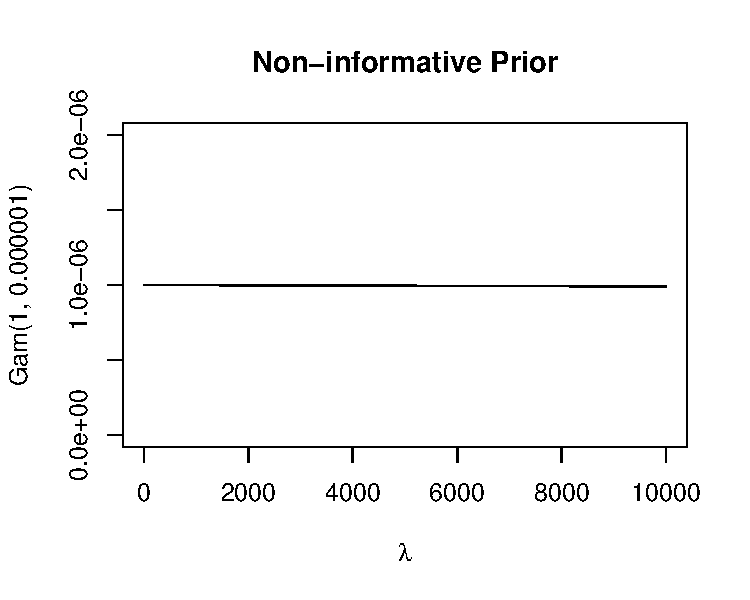
\includegraphics[width=.5\linewidth]{figure/noninform-1} 

\end{knitrout}
\end{center}

\item Suppose I found out that the total number of bird species on each island is no more than $100$, and I found out that in general lower extinction numbers are more likely than higher ones. I could incorporate this knowledge by assigning a weakly informative $Gam(1, 0.02)$ prior, with probabilities generally decreasing between $0$ and $100$. This prior is still vague, but I am incorporating knowledge about a general trend and a natural constraint. I wish I could make values over $100$ have zero probability, but I'm not sure this can be done with the gamma distribution.

\begin{center}
\begin{knitrout}\footnotesize
\definecolor{shadecolor}{rgb}{0.969, 0.969, 0.969}\color{fgcolor}
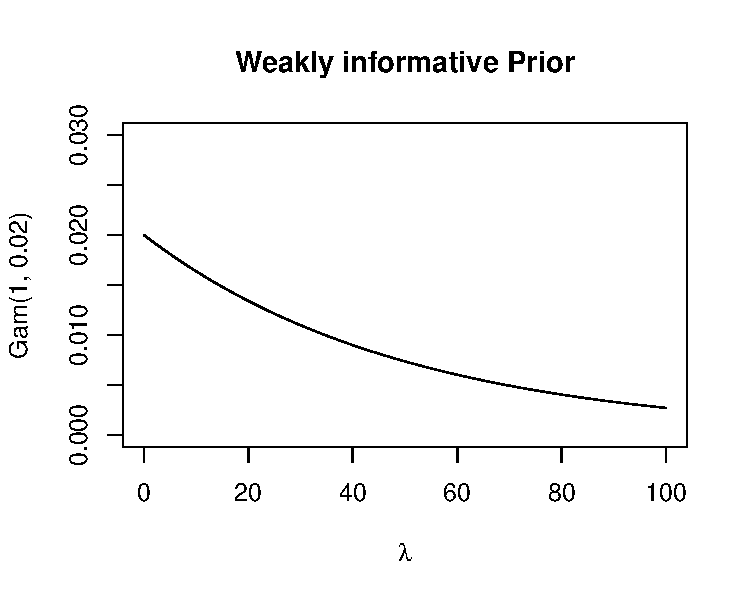
\includegraphics[width=.5\linewidth]{figure/weakinform-1} 

\end{knitrout}
\end{center}

\item I chose the improper $Gam(0, 1)$ prior. This prior gives really high probabilities to low values of $\lambda$ and really low probabilities to values of $\lambda$ greater than $7$ or $8$. 

\begin{center}
\begin{knitrout}\footnotesize
\definecolor{shadecolor}{rgb}{0.969, 0.969, 0.969}\color{fgcolor}
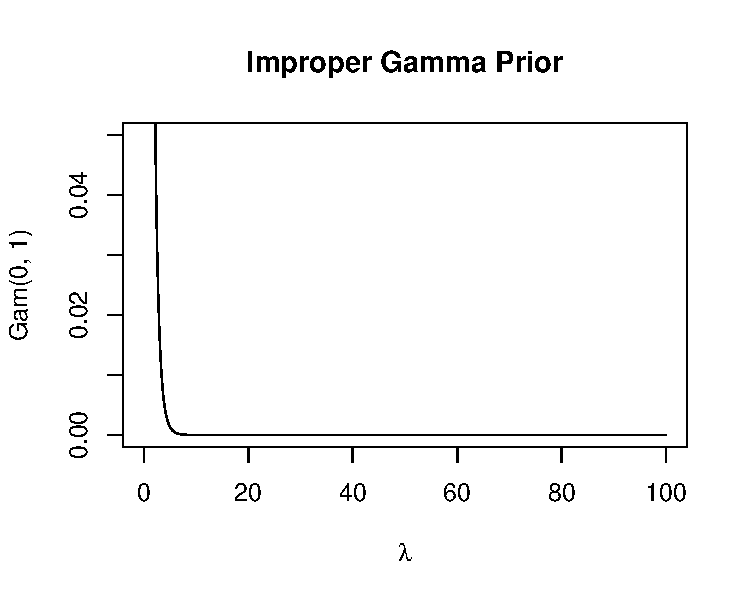
\includegraphics[width=.5\linewidth]{figure/gammaprior-1} 

\end{knitrout}
\end{center}

\item Below are the questions and I asked the researcher and the answers I received:

\begin{enumerate} 
\item {\bf What do you expect the mean number of birds going locally extinct on the island to be?}

{\it Not sure what island specifically you are referring to?  If you're thinking about an average number over all islands, I would guess around 5, but I'm not super confident in that.  We definitely noticed in observations that we weren't seeing species we used to see, but hard to pin it down to one expected number.}

\item {\bf What is your estimated probability that the mean is between 1 and 20?} 
{\it Not quite sure how to assign a probability here -- are you asking if I think it would be rare to have 0 or more than 20 birds go extinct for an island?  I think it would be rare to have more than 20, but I probably wouldn't say it's impossible…just not likely.  An island could have 0 birds go extinct..that's definitely plausible.}

\item {\bf Or, if the last question was easy for you, what is your estimated probability that the mean is between 1 and 10?}

{\it Last question was not so easy for me :)  -- but I would say I think 15 would be really high for an island, and 10 would be fairly high (though would definitely expect it for some of the islands).  I'm not so sure about how to think about "the mean" you're referring to, so these are answers about what I would expect for an island.}
\end{enumerate}

After considering the researcher's answers, and the possible shapes from the gamma distribution, I chose a $Gam(1, 0.1)$ prior. I would have preferred a shape that gave slightly lower probability to $0$, but I couldn't figure out how to get this shape from the gamma distribution without giving a probability of zero to $0$!. I think the $Gam(1, 0.1)$ prior is reasonable. Values of $\lambda$ between $0$ and $10$ are most probable, and values greater than $20$ are less likely but still possible.

\begin{center}
\begin{knitrout}\footnotesize
\definecolor{shadecolor}{rgb}{0.969, 0.969, 0.969}\color{fgcolor}
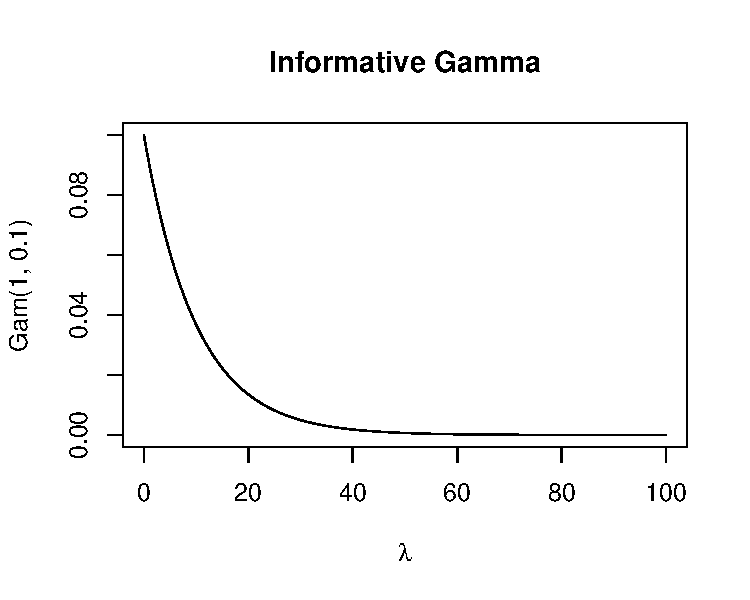
\includegraphics[width=.5\linewidth]{figure/propergamma-1} 

\end{knitrout}
\end{center}

\item I put this together by trial and error. Probabilities generally decrease for higher values of $\lambda$, but values between $0$ and $3$ have lower probability than values between $4$ and $7$. The code is shown below, along with the plot of the prior. 

\begin{center}
\begin{singlespace}
\begin{knitrout}\footnotesize
\definecolor{shadecolor}{rgb}{0.969, 0.969, 0.969}\color{fgcolor}\begin{kframe}
\begin{alltt}
\hlstd{prior.fun} \hlkwb{<-} \hlkwa{function}\hlstd{(}\hlkwc{theta}\hlstd{)\{}
  \hlkwa{if}\hlstd{(theta} \hlopt{<=} \hlnum{3}\hlstd{) \{out} \hlkwb{<-} \hlnum{0.14}\hlopt{/}\hlnum{3}\hlstd{\}}
  \hlkwa{if}\hlstd{(theta} \hlopt{>} \hlnum{3} \hlopt{&} \hlstd{theta} \hlopt{<=} \hlnum{7}\hlstd{) \{out} \hlkwb{<-} \hlnum{0.21}\hlopt{/}\hlnum{4}\hlstd{\}}
  \hlkwa{if}\hlstd{(theta} \hlopt{>} \hlnum{7} \hlopt{&} \hlstd{theta} \hlopt{<=} \hlnum{10}\hlstd{) \{out} \hlkwb{<-} \hlnum{0.13}\hlopt{/}\hlnum{3}\hlstd{\}}
  \hlkwa{if}\hlstd{(theta} \hlopt{>} \hlnum{10} \hlopt{&} \hlstd{theta} \hlopt{<=} \hlnum{15}\hlstd{) \{out} \hlkwb{<-} \hlnum{0.16}\hlopt{/}\hlnum{5}\hlstd{\}}
  \hlkwa{if}\hlstd{(theta} \hlopt{>} \hlnum{15} \hlopt{&} \hlstd{theta} \hlopt{<=} \hlnum{20}\hlstd{) \{out} \hlkwb{<-} \hlnum{0.1}\hlopt{/}\hlnum{5}\hlstd{\}}
  \hlkwa{if}\hlstd{(theta} \hlopt{>} \hlnum{20} \hlopt{&} \hlstd{theta} \hlopt{<=} \hlnum{30}\hlstd{) \{out} \hlkwb{<-} \hlnum{0.11}\hlopt{/}\hlnum{10}\hlstd{\}}
  \hlkwa{if}\hlstd{(theta} \hlopt{>} \hlnum{30} \hlopt{&} \hlstd{theta} \hlopt{<=} \hlnum{40}\hlstd{) \{out} \hlkwb{<-} \hlnum{0.05}\hlopt{/}\hlnum{10}\hlstd{\}}
  \hlkwa{if}\hlstd{(theta} \hlopt{>} \hlnum{40} \hlopt{&} \hlstd{theta} \hlopt{<=} \hlnum{60}\hlstd{) \{out} \hlkwb{<-} \hlnum{0.05}\hlopt{/}\hlnum{20}\hlstd{\}}
  \hlkwa{if}\hlstd{(theta} \hlopt{>} \hlnum{60} \hlopt{&} \hlstd{theta} \hlopt{<=} \hlnum{100}\hlstd{) \{out} \hlkwb{<-} \hlnum{0.05}\hlopt{/}\hlnum{40}\hlstd{\}}
  \hlkwd{return}\hlstd{(out)}
\hlstd{\}}

\hlstd{x} \hlkwb{<-} \hlkwd{seq}\hlstd{(}\hlnum{0}\hlstd{,} \hlnum{100}\hlstd{,} \hlkwc{by}\hlstd{=}\hlnum{0.1}\hlstd{)}
\hlstd{input} \hlkwb{<-} \hlkwd{data.frame}\hlstd{(x)}
\hlstd{probs} \hlkwb{<-} \hlkwd{apply}\hlstd{(input,} \hlnum{1}\hlstd{, prior.fun)}
\hlkwd{plot}\hlstd{(x, probs,} \hlkwc{type}\hlstd{=}\hlstr{"l"}\hlstd{,} \hlkwc{xlab}\hlstd{=}\hlkwd{expression}\hlstd{(lambda),} \hlkwc{main}\hlstd{=}\hlstr{"Stepwise prior"}\hlstd{)}
\end{alltt}
\end{kframe}
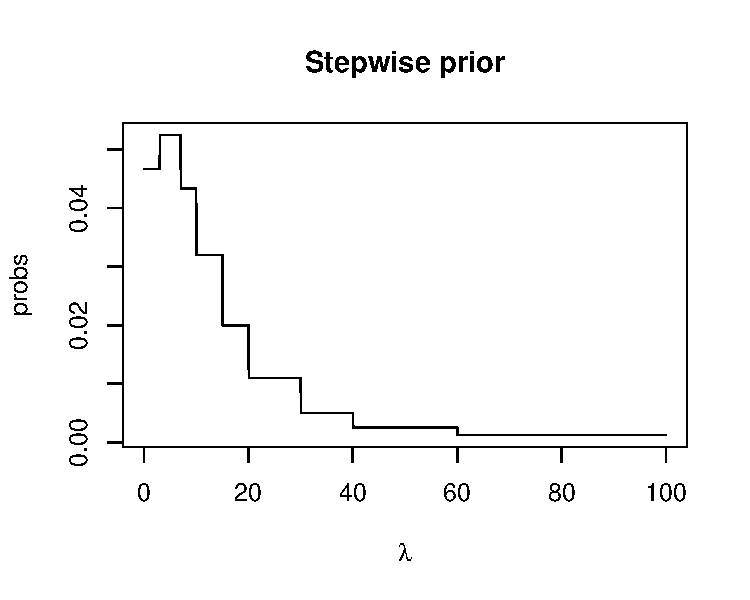
\includegraphics[width=.5\linewidth]{figure/stepprior-1} 
\begin{kframe}\begin{alltt}
\hlcom{#check that it sums to 1}
\hlkwd{sum}\hlstd{(}\hlnum{0.1}\hlopt{*}\hlstd{probs[}\hlopt{-}\hlkwd{c}\hlstd{(}\hlnum{100}\hlstd{)])}
\end{alltt}
\begin{verbatim}
## [1] 1
\end{verbatim}
\end{kframe}
\end{knitrout}
\end{singlespace}
\end{center}

\end{enumerate}

\item The plot below shows all five priors together.

\begin{center}
\begin{knitrout}\footnotesize
\definecolor{shadecolor}{rgb}{0.969, 0.969, 0.969}\color{fgcolor}
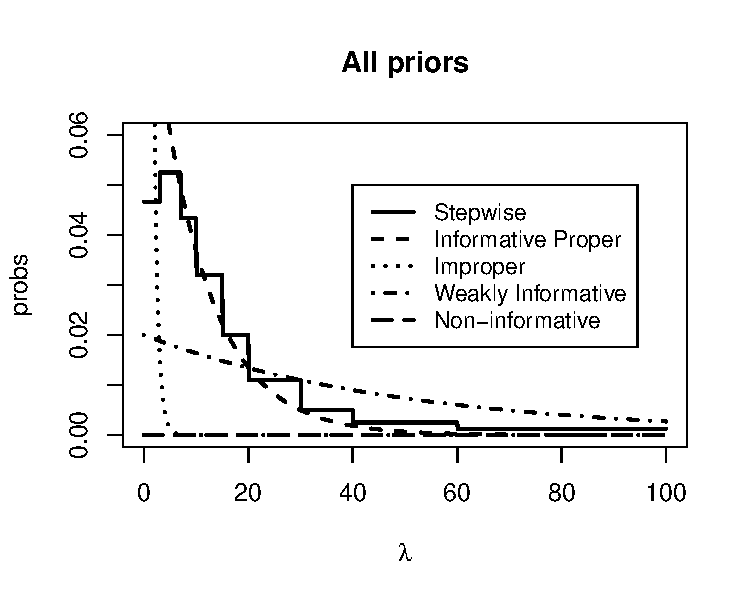
\includegraphics[width=.5\linewidth]{figure/together-1} 

\end{knitrout}
\end{center}

\item The plots of the observed data and the likelihood function are shown below.

\begin{knitrout}\footnotesize
\definecolor{shadecolor}{rgb}{0.969, 0.969, 0.969}\color{fgcolor}
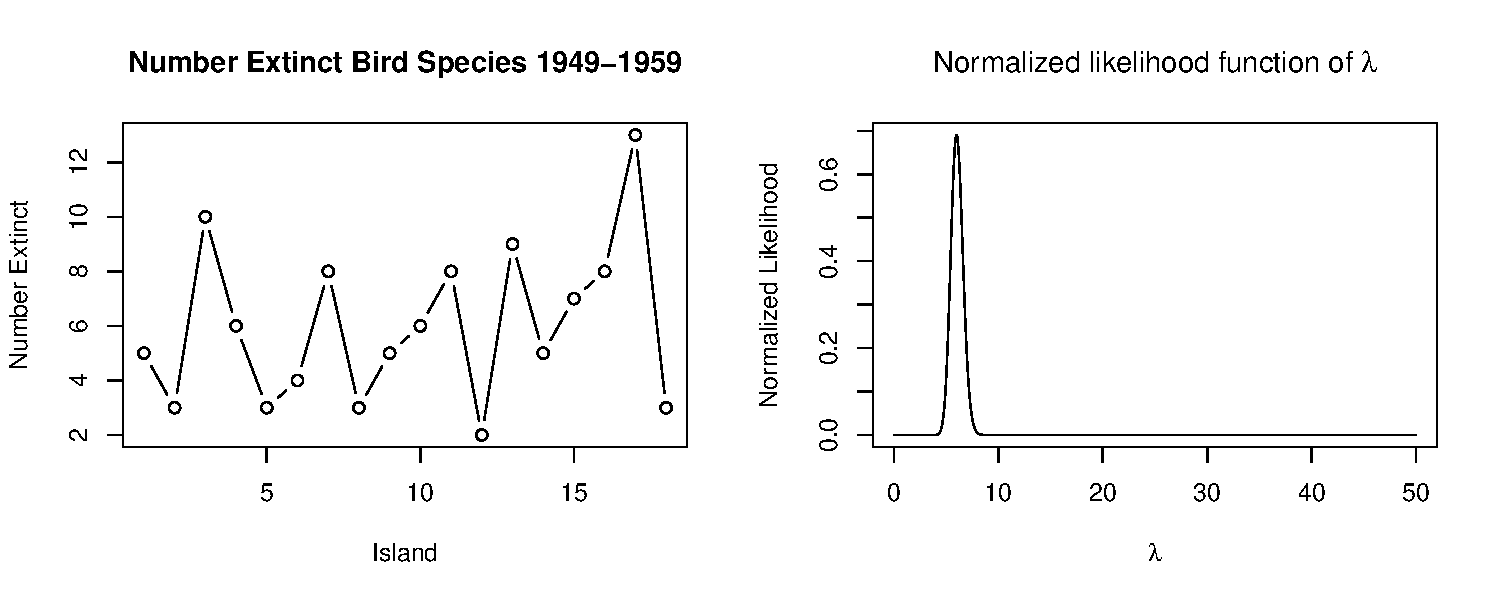
\includegraphics[width=\linewidth]{figure/likefun-1} 

\end{knitrout}


\item On HW 3 I proved mathematically that for a Poisson likelihood and a $Gam(a, b)$ prior, the posterior distribution is $Gam(\sum_{i=1}^n y_i+a, b+n)$. I use this result to find the posterior distributions for priors (i) through (iv).

\begin{enumerate}

\item $Gam(1, 0.000001)$ prior $\rightarrow Gam(108+1, 18+0.000001)$ posterior

\item $Gam(1, 0.02)$ prior $\rightarrow Gam(108+1, 18+0.02)$ posterior

\item $Gam(0, 1)$ prior $\rightarrow Gam(108+0, 18+1)$ posterior

\item $Gam(1, 0.1)$ prior $\rightarrow Gam(108+1, 18+0.1)$ posterior

\item The function used to approximate the posterior probability distribution for $\lambda$ is shown below for the stepwise prior. I found that the posterior distribution for this prior is almost identical to the normalized likelihood function. 



\begin{singlespace}
\begin{knitrout}\footnotesize
\definecolor{shadecolor}{rgb}{0.969, 0.969, 0.969}\color{fgcolor}\begin{kframe}
\begin{alltt}
\hlcom{#likelihood function}
\hlstd{like.pois} \hlkwb{<-} \hlkwa{function}\hlstd{(}\hlkwc{lambda}\hlstd{)\{}
  \hlstd{lambda}\hlopt{^}\hlstd{\{}\hlkwd{sum}\hlstd{(extinctions}\hlopt{$}\hlstd{extinct)\}}\hlopt{*}\hlkwd{exp}\hlstd{(}\hlopt{-}\hlnum{18}\hlopt{*}\hlstd{lambda)}\hlopt{/}\hlkwd{prod}\hlstd{(}\hlkwd{factorial}\hlstd{(extinctions}\hlopt{$}\hlstd{extinct))}
\hlstd{\}}

\hlcom{#Write a function to calculate the posterior probability for each value of lambda}
\hlstd{post.fun} \hlkwb{<-} \hlkwa{function}\hlstd{(}\hlkwc{lambda}\hlstd{) \{}
  \hlkwd{prior.fun}\hlstd{(lambda)}\hlopt{*}\hlkwd{like.pois}\hlstd{(lambda)}
\hlstd{\}}

\hlcom{#Look at lambdas between 0 and 10}
\hlstd{lambda} \hlkwb{<-} \hlkwd{seq}\hlstd{(}\hlnum{0}\hlstd{,} \hlnum{10}\hlstd{,} \hlkwc{by}\hlstd{=}\hlnum{0.001}\hlstd{)}

\hlcom{#Normalize the posterior distribution}
\hlstd{numint.post} \hlkwb{<-} \hlkwd{sum}\hlstd{(}\hlnum{0.001}\hlopt{*}\hlkwd{post.fun}\hlstd{(lambda))}
\hlstd{post.probs} \hlkwb{<-} \hlkwd{post.fun}\hlstd{(lambda)}\hlopt{/}\hlstd{numint.post}
\end{alltt}
\end{kframe}
\end{knitrout}
\end{singlespace}

\begin{center}
\begin{knitrout}\footnotesize
\definecolor{shadecolor}{rgb}{0.969, 0.969, 0.969}\color{fgcolor}
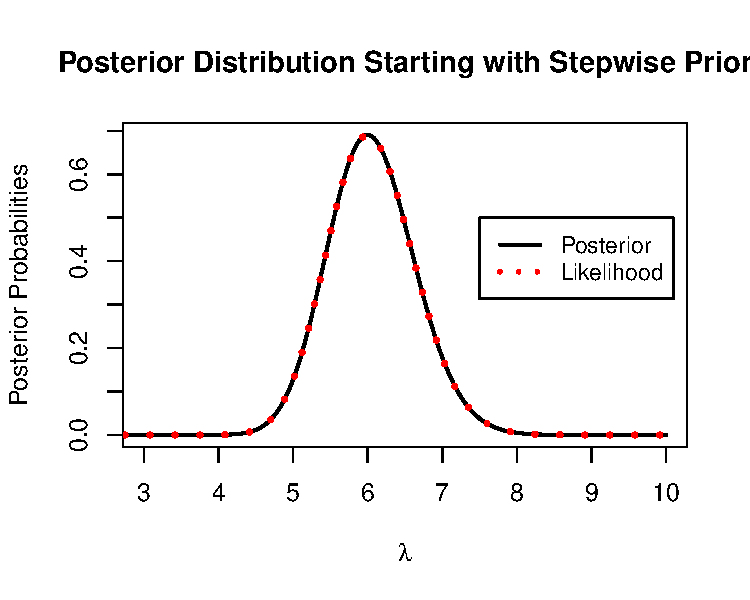
\includegraphics[width=.5\linewidth]{figure/plotting-1} 

\end{knitrout}
\end{center}

\end{enumerate}

\item The posterior probabilities and intervals are shown for each posterior in the table below. My code for approximating these quantities for the posterior distribution found computationally are shown below.



\begin{singlespace}
\begin{knitrout}\footnotesize
\definecolor{shadecolor}{rgb}{0.969, 0.969, 0.969}\color{fgcolor}\begin{kframe}
\begin{alltt}
\hlkwd{require}\hlstd{(mosaic,} \hlkwc{quietly}\hlstd{=}\hlnum{TRUE}\hlstd{)}
\hlkwd{set.seed}\hlstd{(}\hlnum{49}\hlstd{)}
\hlstd{post.samp} \hlkwb{<-} \hlkwd{sample}\hlstd{(lambda,} \hlnum{10000}\hlstd{,} \hlkwc{prob}\hlstd{=post.probs,} \hlkwc{replace}\hlstd{=}\hlnum{TRUE}\hlstd{)}
\hlkwd{quantile}\hlstd{(post.samp,} \hlnum{0.005}\hlstd{)}
\hlkwd{quantile}\hlstd{(post.samp,} \hlnum{0.995}\hlstd{)}
\hlnum{1}\hlopt{-}\hlkwd{pdata}\hlstd{(}\hlnum{5}\hlstd{, post.samp)}
\end{alltt}
\end{kframe}
\end{knitrout}
\end{singlespace}

\begin{table}[H]
\centering
\begin{tabular}{c|c|c|c}
Prior & Posterior & 99\% Post Interval & Post Prob $>$ 5 \\
\hline
Gam(1, 0.000001) & Gam(109, 18.000001) & (4.666, 7.654) & 0.972 \\
Gam(1, 0.02) & Gam(109, 18.02) & (4.661, 7.645) & 0.971 \\
Gam(0, 1) & Gam(108, 19) & (4.374, 7.192) & 0.898 \\
Gam(1, 0.1) & Gam(109, 18.1) & (4.640, 7.611) & 0.968 \\
Stepwise & shown above & (4.672, 7.655) & 0.970 \\
\hline
\end{tabular}
\end{table}

\item The results are similar across the non-informative, weakly informative, informative ($Gam(1, 0.1)$), and stepwise priors. I think that the posterior distributions for the non-informative and weakly informative priors are similar to the stepwise and $Gam(1, 0.1)$ informative priors because these informative priors turned out to be consistent with the data observed. The one prior that gave different results was the improper $Gam(0, 1)$ prior. The improper $Gam(0, 1)$ prior is highly informative, giving very high weight to small values of $\lambda$. This prior clearly influenced the posterior distribution in this example by drawing more density towards lower values of $\lambda$. In this case, I believe that the information provided by the improper Gamma prior was incorrect, and I don't trust the results from the Gamma prior as much as I trust the results from the other priors. I think this shows that it is better to incorporate more uncertainty into a prior rather than choosing a highly informative prior that may be incorrect.

%The posterior distribution is sensitive to the choice of {\it informative} prior.

\item The approximate posterior predictive distribution found starting from the stepwise prior is shown below. Here are the steps I went through to construct the approximation:
\begin{itemize}
\item Draw a random $\lambda$ from the approximate posterior distribution found in part (e). To do this, I use the sample function to sample from the $\lambda$ vector with probabilities equal to the posterior probabilities found in part (e).
\item Draw a random observation from a $Poi(\lambda)$ distribution where $\lambda$ is the one you drew above. 
\item Repeat steps $1$ and $2$ $10000$ times. Note: Computationally, I did it with vectors, but for understanding I think it makes more sense to explain it this way.
\item Ignore $\lambda$ for each pair and plot the observations. This is the approximate posterior predictive distribution.
\end{itemize}

\begin{center}
\begin{knitrout}\footnotesize
\definecolor{shadecolor}{rgb}{0.969, 0.969, 0.969}\color{fgcolor}
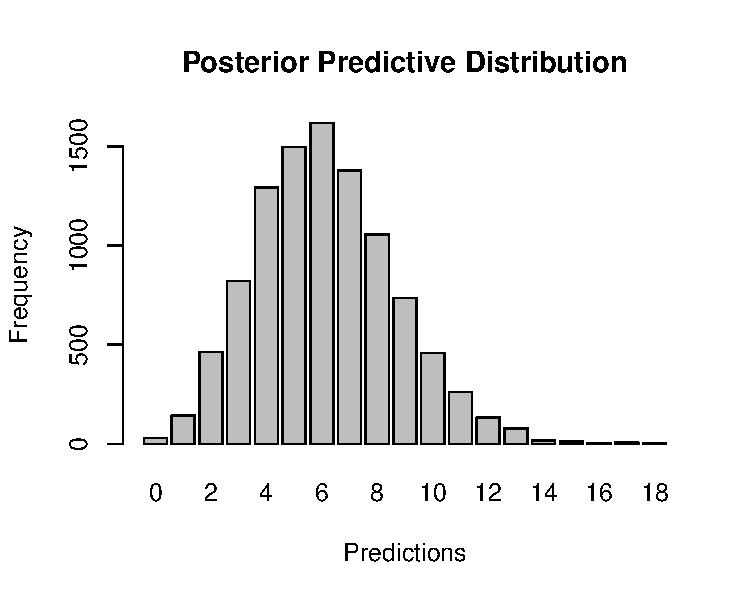
\includegraphics[width=.5\linewidth]{figure/postpred-1} 

\end{knitrout}
\end{center}


\item This ratio is of particular interest because the mean of the observations is assumed to be the same as the variance of the observations when assuming a Poisson model for the data generating process. In the posterior predictive samples, the predictions were generated under the assumption of variance equal to the mean, so the ratios of the sample variances to the sample averages for the posterior predictions should be centered around $1$. If they weren't centered around $1$, I would suspect that I did something wrong when generating the posterior predictions. In the observed data, however, I identified multiple violations of assumptions in the first part of this problem that could manifest as overdispersion. As a result, I am not surprised that the sample variance in the observed data is larger than the sample average. This does not provide evidence of overdispersion, however, because the original ratio of $1.43$ or more extreme was observed $16.8\%$ of the time when data were generated from a true Poisson process. This is a useful modeling check because if the observed ratio was way out in the tails of the below distribution, it would suggest that we should go back and rethink the model used to describe the data generating process.

\begin{center}
\begin{knitrout}\footnotesize
\definecolor{shadecolor}{rgb}{0.969, 0.969, 0.969}\color{fgcolor}
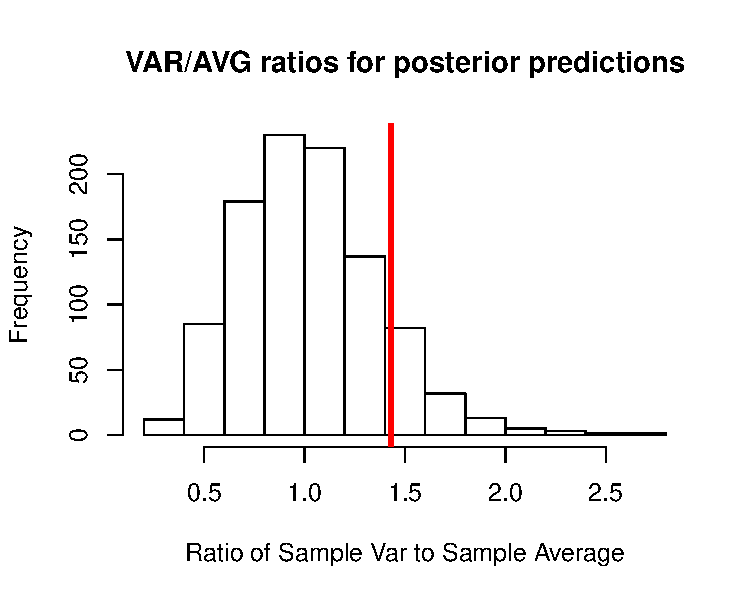
\includegraphics[width=.5\linewidth]{figure/postsamp-1} 

\end{knitrout}
\end{center}

\end{enumerate}

\item \begin{enumerate}

\item I will assume a binomial data generating process where each response is a binomial count of the number of days where an egg was laid in $14$ days. The parameter, $\theta$, is the probability of laying an egg in a day. I'd like to say that I think it is more appropriate to use a poisson process here, but because they want to estimate the probability of laying an egg in a day, I am going to use a binomial process. Most of the assumptions are not met.
\begin{align*}
y_i &\sim Binom(\theta, 14) \\
f(y_i) &= {14 \choose y_i}\theta^{y_i}(1-\theta)^{14-y_i}
\end{align*}
Assumptions:
\begin{itemize}
\item A hen will only lay $0$ or $1$ eggs in a day. She will never lay more than $1$ egg in a day. This makes it so that each day is a binary response going into the binomial count. If she could lay two or more eggs in a day, it wouldn't be appropriate to use a binomial process.
\item Every hen has the same probability of laying an egg in a day. The description acknowledges that this assumption is not met, but they want to estimate an overall probability.
\item There is independence among days for each hen, so that if a hen lays an egg on day one it does not affect the probability of her laying an egg on subsequent days. I don't think this one is met. Biologically, if a hen lays an egg on day one, I expect she would be less likely to lay an egg on day two.
\item There is independence among hens so that if hen $1$ lays an egg, this does not affect the probability of the other hens laying eggs. I think we'd need more information to assess this assumption. There could be some spatial dependence among the hens if their roosts are in close proximity.
\end{itemize}

\item I think a $Beta(1, 1)$ distribution is most appropriate. At first, I wanted to choose a $Beta(2, 2)$ distribution so that the most probable prior value of $\theta$ would be $0.5$, but I couldn't figure out how to get this same shape out of a Beta distribution without completely ruling out the possibility of $\theta$ being $0$ or $1$. In the last problem, I saw that it was better to choose a weakly informative prior rather than a more informative one that might be incorrect. I think biologically it {\it is} possible that a hen could lay $0$ or $14$ eggs in the two week period. The $Beta(1, 1)$ prior allows for this possibility and is a conjugate prior for the binomial likelihood. With a sample size of $60$, I do not think that the resulting posterior distribution will be affected much by the fact that we did not incorporate the researcher's prior knowledge that hens lay an egg every other day on average.

\begin{center}
\begin{knitrout}\footnotesize
\definecolor{shadecolor}{rgb}{0.969, 0.969, 0.969}\color{fgcolor}
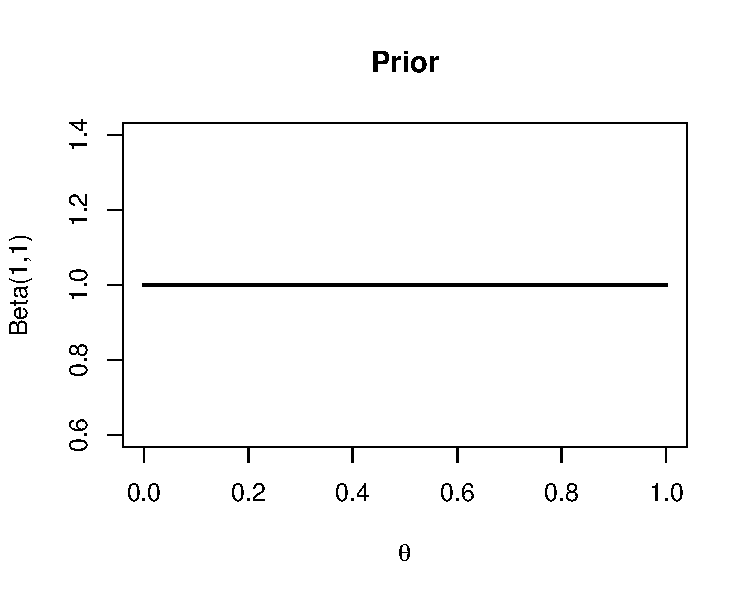
\includegraphics[width=.5\linewidth]{figure/beta22-1} 

\end{knitrout}
\end{center}

\item The data are plotted below. You can see that the sample proportion of days where an egg was laid ranges between $0$ and $0.86$ for different hens.

\begin{center}
\begin{knitrout}\footnotesize
\definecolor{shadecolor}{rgb}{0.969, 0.969, 0.969}\color{fgcolor}
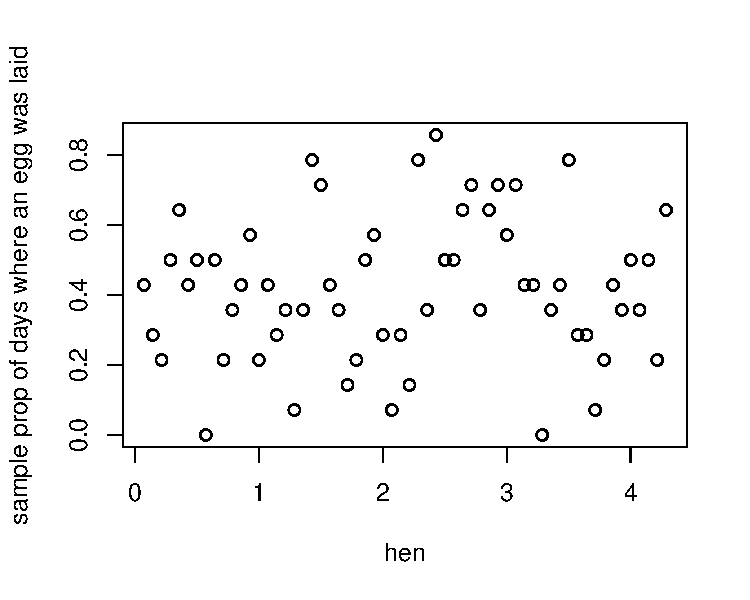
\includegraphics[width=.5\linewidth]{figure/plotdata-1} 

\end{knitrout}
\end{center}

The total number of days where eggs were laid, over all hens, is $349$. The total number of days where eggs were not laid, over all hens, is $491$. In homework $2$ we showed that for a $Beta(a, b)$ prior and a $Binom(n, \theta)$ likelihood, the posterior distribution is $Beta(\sum_{i=1}^n y_i + a, b + \sum_{i=1}^n (n-y_i))$. So, with a $Beta(1, 1)$ prior, the posterior distribution is $Beta(349+1, 491+1)$. The normalized likelihood, prior, and posterior are shown on the plot below.

\begin{center}
\begin{knitrout}\footnotesize
\definecolor{shadecolor}{rgb}{0.969, 0.969, 0.969}\color{fgcolor}
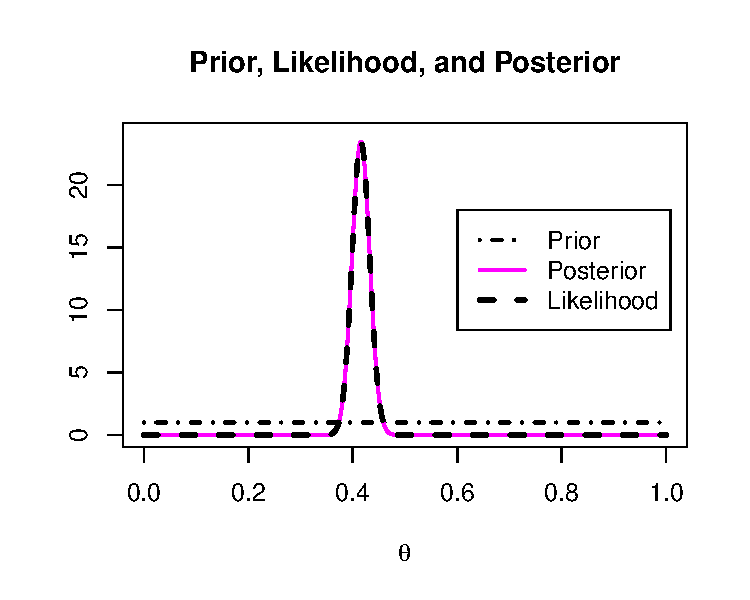
\includegraphics[width=.5\linewidth]{figure/all3-1} 

\end{knitrout}
\end{center}

\item If we use a $Beta(350, 492)$ prior for analyzing the second two week session of data collection, then the posterior for this two week session would be $Beta(365+350, 475+492)$. This prior and posterior are shown on the plot below. I understand why this prior could be justified, because knowledge from a previous study should be used to reflect prior knowledge in subsequent studies. But, I think the posterior from session $1$ is too narrow to use as a prior. I think it puts a lot of weight on the data from session $1$ and almost completely rules out values of $\theta$ less than $0.35$ and greater than $0.5$. 

\begin{center}
\begin{knitrout}\footnotesize
\definecolor{shadecolor}{rgb}{0.969, 0.969, 0.969}\color{fgcolor}
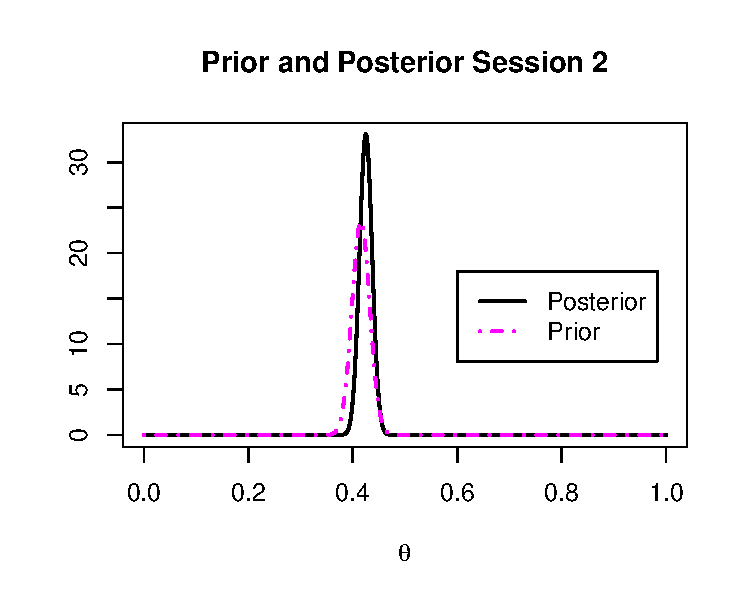
\includegraphics[width=0.6\linewidth]{figure/priortopost-1} 

\end{knitrout}
\end{center}

\item Now I wil use a $Beta(715, 967)$ prior for analyzing the third session of data collection. The posterior for the third session will be $Beta(365+715, 475+967)$. The progression of knowledge is shown below.

\begin{center}
\begin{knitrout}\footnotesize
\definecolor{shadecolor}{rgb}{0.969, 0.969, 0.969}\color{fgcolor}
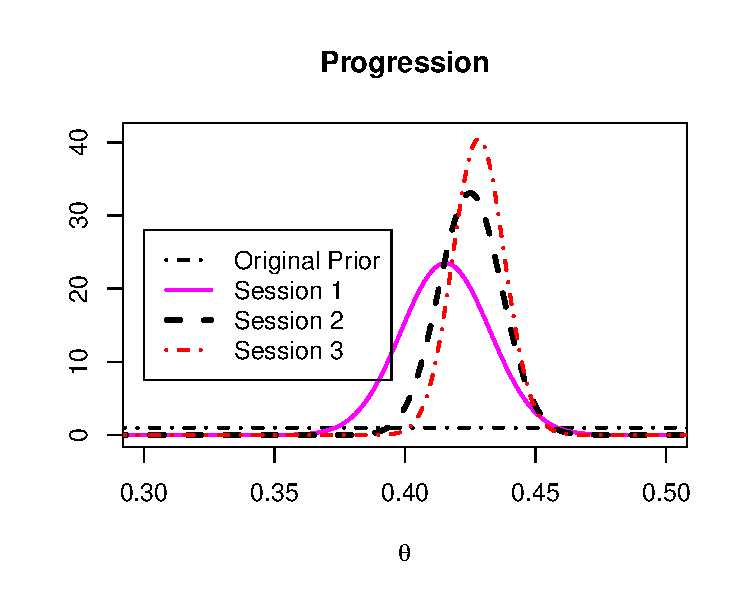
\includegraphics[width=0.8\linewidth]{figure/progress-1} 

\end{knitrout}
\end{center}

\item \begin{enumerate}

\item To make the prior weaker, I simply divide the number of (previous) posterior successes and failures by four. This gives me a prior distribution of $Beta(88, 123)$ for Session $2$. Dividing the posterior parameters from Session $1$ by four keeps the distribution centered at the same value, but it spreads the distribution out more, resulting in a weaker prior. I think the prior used here is much more reasonable than using the exact posterior from Session $1$. By incorporating more uncertainty into the previously found posterior, we don't rule out so many values for $\theta$, but we still incorporate knowledge from the previous session. Under this prior, the posterior distribution for Session $2$ is $Beta(453, 498)$.

\begin{center}
\begin{knitrout}\footnotesize
\definecolor{shadecolor}{rgb}{0.969, 0.969, 0.969}\color{fgcolor}
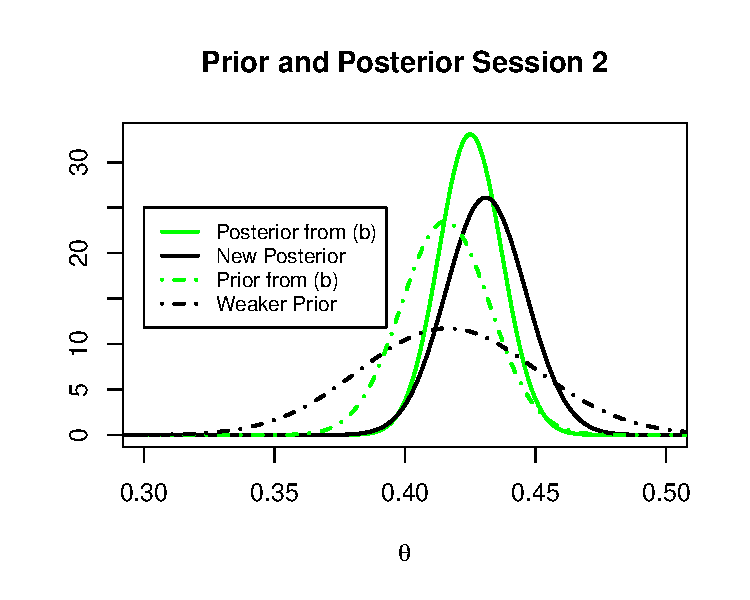
\includegraphics[width=0.6\linewidth]{figure/priortopost2-1} 

\end{knitrout}
\end{center}

\item For session $3$, I take the posterior from session $2$ and divide the parameters by two. I only divide in half this time because I trust the posterior from the second session more than I trust the posterior from the first session; it now reflects knowledge from two studies rather than one. The prior distribution for Session $3$ is then $Beta(227, 299)$ and the posterior distribution for Session $3$ is $Beta(592, 774)$.

\end{enumerate}

\item The progression is shown below. I zoomed in a bit so you could make out the details.

\begin{center}
\begin{knitrout}\footnotesize
\definecolor{shadecolor}{rgb}{0.969, 0.969, 0.969}\color{fgcolor}
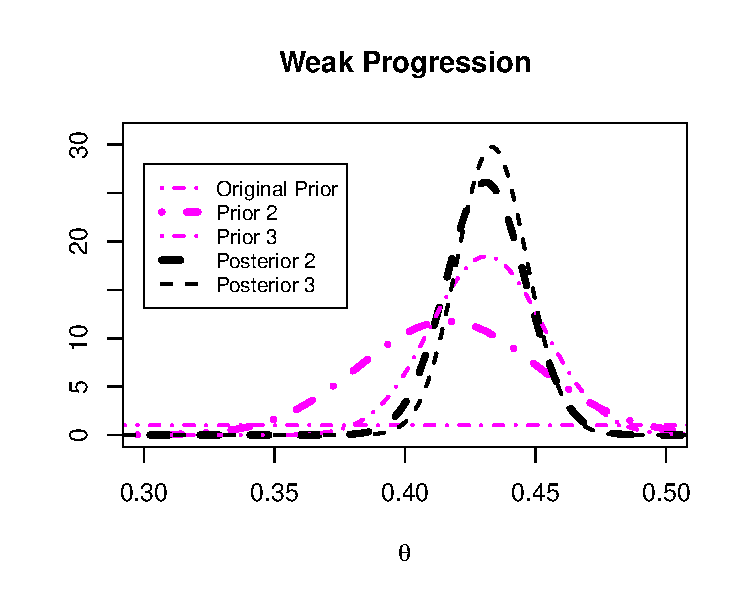
\includegraphics[width=0.7\linewidth]{figure/progress2-1} 

\end{knitrout}
\end{center}

\item If we combine all the data over three time periods, there were $1079$ days on which eggs were laid, and $1441$ days on which eggs were not laid (over all hens). If we start with a $Beta(1, 1)$ prior, then the posterior distribution is $Beta(1079+1, 1441+1)$. The posteriors found in the previous parts are shown on the following plot, along with the posterior found by combining the three time periods into a single dataset. \\

As you can see, the posterior distribution is the same whether we combine the three sessions into a single dataset or whether we find the posterior from each session and use it as the prior for the next session. Wow! The posterior is different, however, if we weaken the posterior from previous sessions before using them as priors for the next session. I still stand by what I said before. The first two posteriors put a lot of weight on the observed data. I think we should take advantage of the fact that the study was repeated three times, and use this opportunity to incorporate uncertainty at each stage. I think the posterior from the weak progression should be used for inference. It is also more conservative, and I generally choose to report the more conservative results.

\begin{center}
\begin{knitrout}\footnotesize
\definecolor{shadecolor}{rgb}{0.969, 0.969, 0.969}\color{fgcolor}
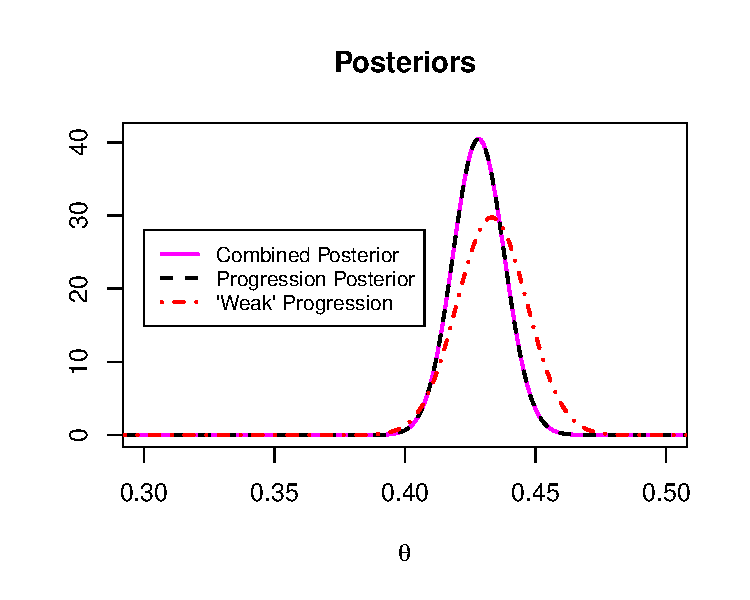
\includegraphics[width=.5\linewidth]{figure/allposterior-1} 

\end{knitrout}
\end{center}

\item I would account for covariates in the estimation of $\theta$ by using a regression equation to predict values of $\theta$ for given values of the covariates. My proposed model is below. We can assign priors and find posteriors for the regression parameters $\beta_0$, $\beta_1$, and $\beta_2$. 
\begin{align*}
y &\sim Binom(\hat{\theta}, 14) \\
\hat{\theta} &= \beta_0+\beta_1I_{fat}+\beta_2I_{M} \\
\beta_0 &\sim Unif(0, 1) \\
\beta_1 &\sim Unif(-1, 1) \\
\beta_2 &\sim Unif(-1, 1)
\end{align*}
where $I_M$ is $1$ if the hen is molting and $0$ if not, and $I_{fat}$ is $1$ if eating more than $80$ grams of food per day, and $0$ if otherwise. \\

The first covariate is a measure of the the amount of food the birds eat each day. I made this an indicator variable so that it would be easy to put a prior on the coefficient associated with it, $\beta_1$. $\beta_1$ represents the difference in probabilities of laying an egg between hens that eat more than $80$ grams of food per day and hens that eat less than or equal to 80 grams. I know nothing about hens and how food consumption is related to egg laying, so I will put a $Unif(-1, 1)$ prior on $\beta_1$ to allow for the possibility that an increase in food intake is associated with an increase or a decrease in the probability of laying an egg. \\

%Google says that birds eat about $100$ grams of food per day when they are laying, and only about $70$ grams of food per day when they aren't laying (I figured Google was OK here because it's not content related). So, I'd estimate that a food consumption increase of $10$ grams is associated with a $0.3$ increase in the probability of laying an egg. This means my best guess of $\beta_1$ is $0.3$, but I'm not very confident in this estimate and I'd like to allow for the possibility that an increase in food intake is actually associated with a decrease in the probability of laying an egg. I'll put a $N(0.3, 0.15)$ on $\beta_1$. I realize it's a little strange, because it does allow for the possibility of getting a completely impossible value such as $1.5$, but I didn't know what distribution I could use (other than a uniform) that would only allow for values between $-1$ and $1$. A uniform didn't seem appropriate because I couldn't incorporate the knowledge that $\beta_1$ is near $0.3$. \\


The second covariate is an indicator variable that is $1$ if they are molting and $0$ if they are not. $\beta_2$ is then the difference in the probability of laying an egg in a day between molting hens and non-molting hens. I have no idea whether molting hens are more likely to lay eggs than non-molting hens, so I will put a $Unif(-1, 1)$ prior on $\beta_2$. \\

%I think that hens generally do not lay eggs when they are molting. So, $\beta_2$ is expected to be a negative number. If we start with the assumption that the probability of laying an egg is around $0.5$ when non-molting, and expect the probability of laying an egg when molting to be near $0$, they I would expect the value of $\beta_2$ to be near $-0.5$. I'd like to allow for values near $-0.5$ to be probable, and I don't want to completely rule out small positive numbers. I think a $N(-0.5, 0.15)$ distribution is the best choice here. Again, refer to my comment above about using a normal distribution in this situation.


$\beta_0$ is the value of $\theta$ when they are not molting and when they are eating $0$ pounds of food per day. Because I don't know anything about the effect of food consumption and molting on the probability of laying an egg, I'll use a non-informative $Unif(0,1)$ prior for $\beta_0$ as well.

\begin{knitrout}\footnotesize
\definecolor{shadecolor}{rgb}{0.969, 0.969, 0.969}\color{fgcolor}
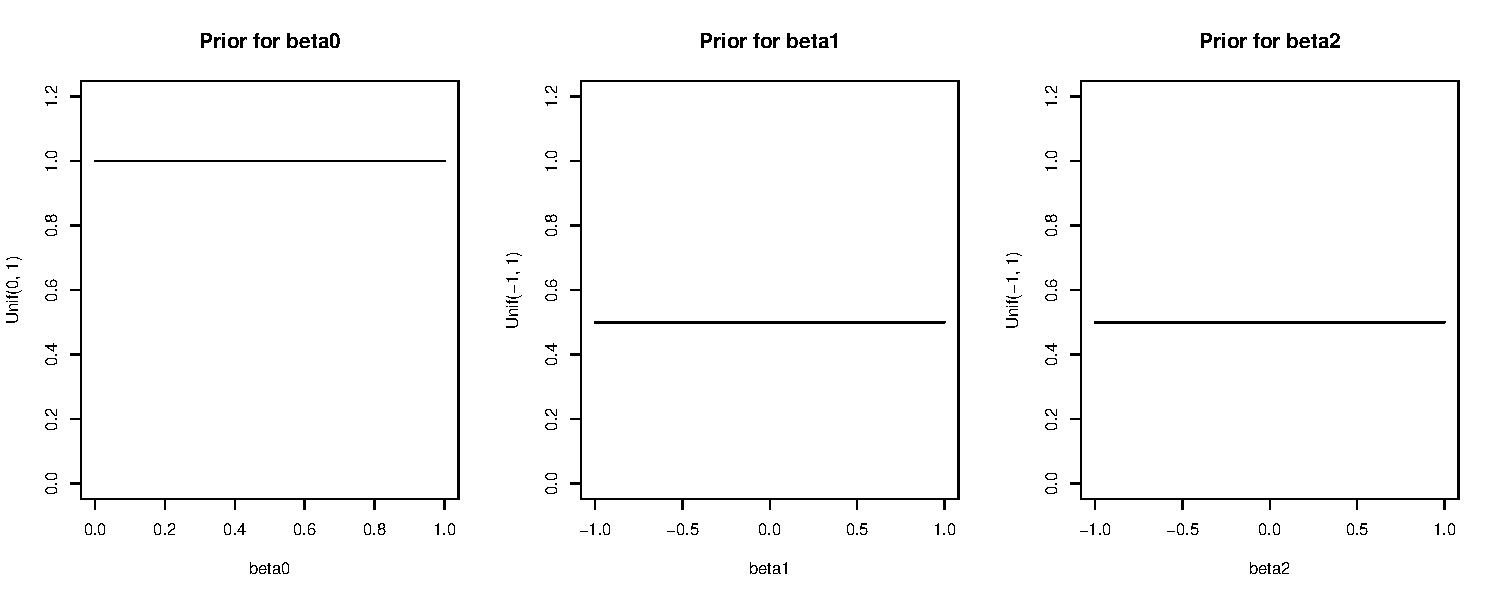
\includegraphics[width=\linewidth]{figure/plotprs-1} 

\end{knitrout}


\end{enumerate}

\end{enumerate}

\end{doublespacing}

\end{document}
